\chapter{Comparisons}

\newcommand*\rot{\rotatebox{90}}

\afterpage{
    \thispagestyle{empty}
    \begin{sidewaystable}
        \centering
        \begin{tabular}{r l l l l l l}
            \toprule
             & \rot{First Release} & \rot{Latest Release} & \rot{Latest Version} & \rot{Platforms} & \rot{\shortstack[l]{Programming\\Languages}} & \rot{\shortstack[l]{Scripting\\Languages}} \\
            \midrule
             Blender Game Engine & 2000 & 09/2017 & 2.79 & W/L/M & C, C++, Python & Python \\
             CryEngine & 03/2002 & 09/2018 & 5.5 & W/L & C++ & Lua, C\# \\
             %Frostbite & 06/2008 & 10/2011 & 3 & W & C++, C\# & -\\
             %id Tech & 05/2016 & 05/2016 & 6 & W & C++ & - \\
             Source & 06/2004 & - & - & W/L/M & C++\cite{SourceValveDeveloperCommunity} & C++ \\
             Unity 3D & 06/2005 & 12/2018 & 2018.3 & W/L/M & C++ & C\# \\
             Unreal & 05/1998 & 11/2018 & 4 & W/L/M & C++ & C++, Blueprints \\
            \bottomrule
        \end{tabular}
        \captionof{table}{Comparison of Popular Game Engines}
        \label{table:game-engines}
    \end{sidewaystable}
}

\chapter{Algorithms}
\begin{algorithm}[H]
    \SetKwData{MutationManager}{mutationManager}\SetKwData{RecordingManager}{recordingManager}\SetKwData{RobotController}{robotController}
    \SetKwFunction{AlterScene}{AlterScene}\SetKwFunction{CaptureRecord}{CaptureRecord}\SetKwFunction{MutationCompleted}{MutationCompleted}\SetKwFunction{ResetScene}{ResetScene}\SetKwFunction{Move}{Move}\SetKwFunction{DestinationReached}{DestinationReached}
    
    \Repeat{not \DestinationReached{\RobotController}}{
        \Repeat{not \MutationCompleted{\MutationManager}}{
            \AlterScene{\MutationManager}\;
            \CaptureRecord{\RecordingManager}\;
        }
        \ResetScene{\MutationManager}\;
        \Move{\RobotController}\;
    }
    
    \caption{Fully Automatic Mode}\label{algo:automatic-mode}
\end{algorithm}

\begin{algorithm}[H]
    \SetKwData{StepSize}{stepSize}\SetKwData{Findings}{findings}\SetKwData{Region}{region}\SetKwData{Ray}{ray}\SetKwData{Hit}{hit}\SetKwData{Collider}{collider}\SetKwData{ScreenPosition}{screenPosition}
    \SetKwFunction{ScreenPointToRay}{ScreenPointToRay}\SetKwFunction{ExtendRectangle}{ExtendTo}\SetKwFunction{Vector}{Vector}\SetKwFunction{Map}{Map}\SetKwFunction{Rectangle}{Rectangle}\SetKwFunction{Contains}{Contains}\SetKwFunction{Get}{Get}\SetKwFunction{Set}{Set}\SetKwFunction{HasHit}{HasHit}\SetKwFunction{GetCollider}{GetCollider}\SetKwFunction{GetHit}{GetHit}\SetKwFunction{GetCollider}{GetCollider}\SetKwFunction{GetX}{GetX}\SetKwFunction{GetY}{GetY}
    \SetKwInOut{Input}{input}\SetKwInOut{Output}{output}
    \Input{Scan-resolution as $wScan$ and $hScan$, screen-resolution as $wScreen$ and $hSreen$ and the $camera$ used}
    \Output{Findings}
    \BlankLine
    \StepSize $\leftarrow$ \Vector{$\dfrac{wScreen}{wScan}, \dfrac{hScreen}{hScan}$}\;
    \Findings $\leftarrow$ \Map{}\;
    
    \For{$x \leftarrow 0$ \KwTo $wScan + 1$} {
        \For{$y \leftarrow 0$ \KwTo $hScan + 1$} {
    		\ScreenPosition $\leftarrow$ \Vector{$\GetX{\StepSize} \times x$, $\GetY{\StepSize} \times y$}\;
    		\Ray $\leftarrow$ \ScreenPointToRay{$camera$, \ScreenPosition}\;
    		\If{\HasHit{\Ray}}{
    		    \Collider $\leftarrow$ \GetCollider{\GetHit{\Ray}}\;
        		\Region $\leftarrow$ \Rectangle{}\;
    			\If { $\Contains{\Findings, \Collider}$ } { 
    			    \Region $\leftarrow$ \Get{\Findings, \Collider}\;
        		}
    			\If { $not \Contains{\Region, \ScreenPosition}$} {
    			    \ExtendRectangle{\Region, \ScreenPosition}\;
    			}
    			\Set{\Findings, \Collider, \Region}\;
    		}
    	}
    }
    \KwRet{\Findings}
    \caption{Raycasting from screen-space}\label{algo:raycasting-screenspace}
    \SetAlCapSkip{1em}
\end{algorithm}

\chapter{Diagrams}
\begin{sidewaysfigure}
    \centering
    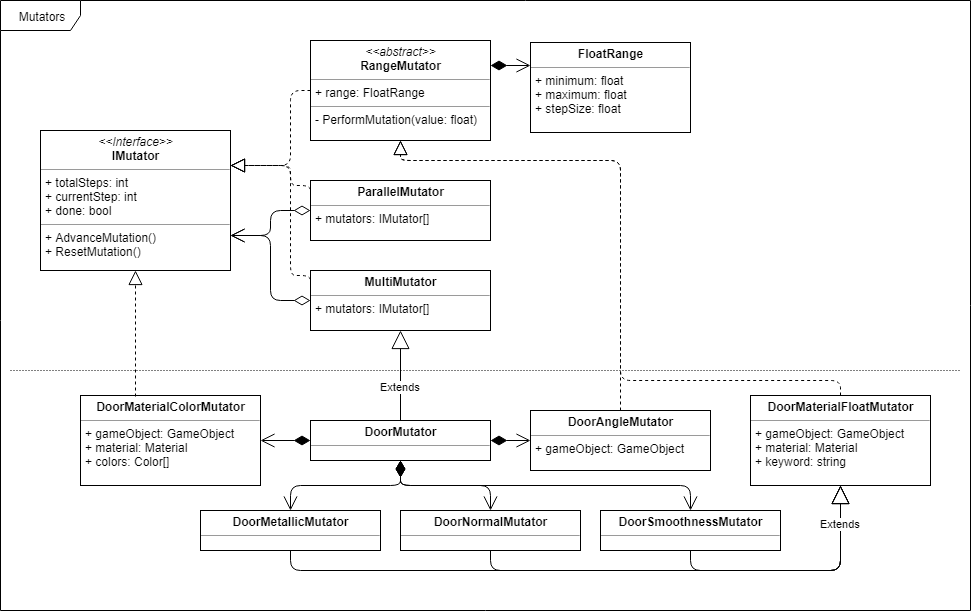
\includegraphics[height=350pt]{img/ch05/ClassDiagram_Mutators_Door03.png}
    \captionof{figure}[Mutators class diagram]{Mutator-interfaces and the exemplaric implementation of door-mutators}
    \label{fig:classdiagram-mutators}
\end{sidewaysfigure}

\chapter{Generated Output}
\label{chap:appendix-output}
\begin{sidewaysfigure}
    \centering
    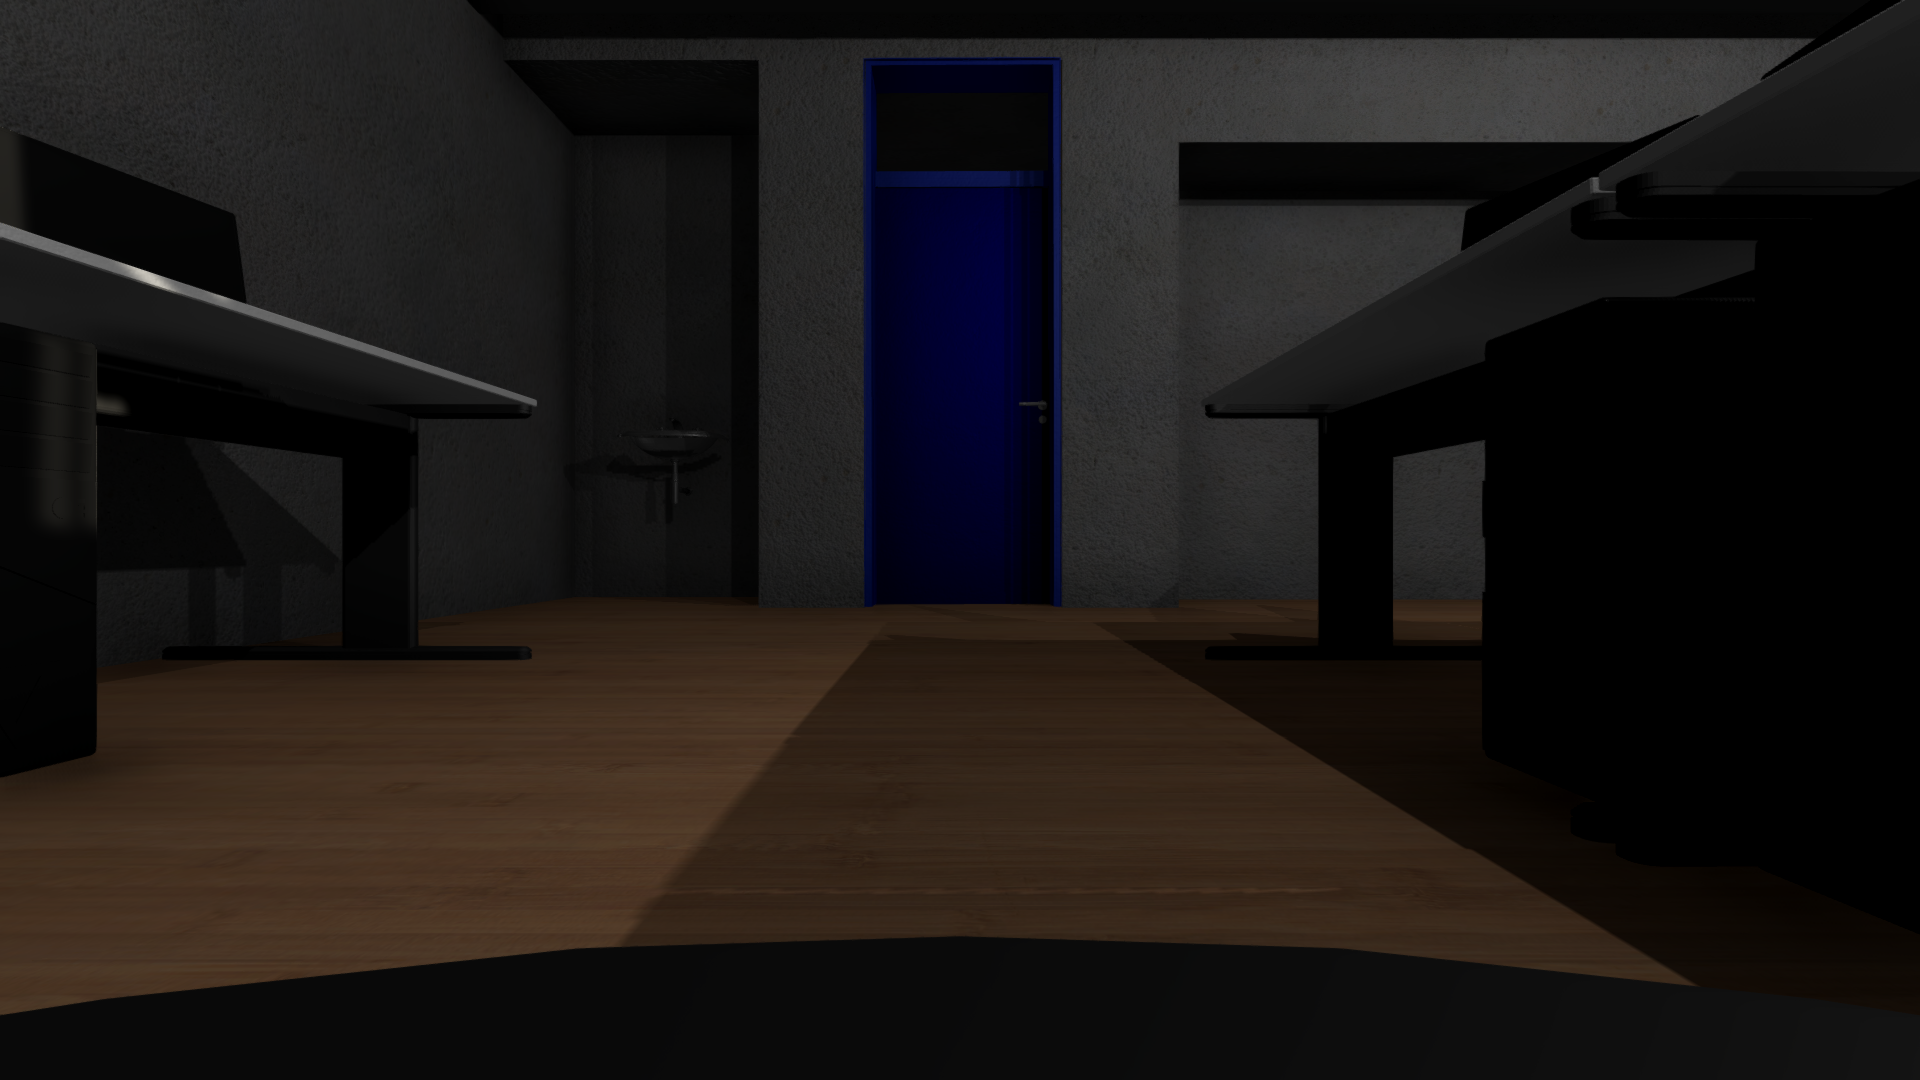
\includegraphics[height=350pt]{appendix/P3AT_Test1_2019-01-22_18-28-07_454.png}
    \captionof{figure}[1080p Output Image]{Rendered image with $1980 \times 1080$ pixels}
    \label{fig:output-image}
\end{sidewaysfigure}
\begin{listing}[ht]
    \inputminted{json}{appendix/P3AT_Test1_2019-01-22_18-28-07_454.meta.json}
    \caption{The generated meta file to \ref{fig:output-image} (shortened)}
    \label{listing:output-meta}
\end{listing}
\begin{listing}[ht]
\inputminted{text}{appendix/P3AT_Test1_2019-01-22_18-28-07_454.txt}
    \caption{The generated text file to \ref{fig:output-image} for use with the \textit{"Darknet"} framework}
    \label{listing:output-json}
\end{listing}
\begin{sidewaysfigure}
    \centering
    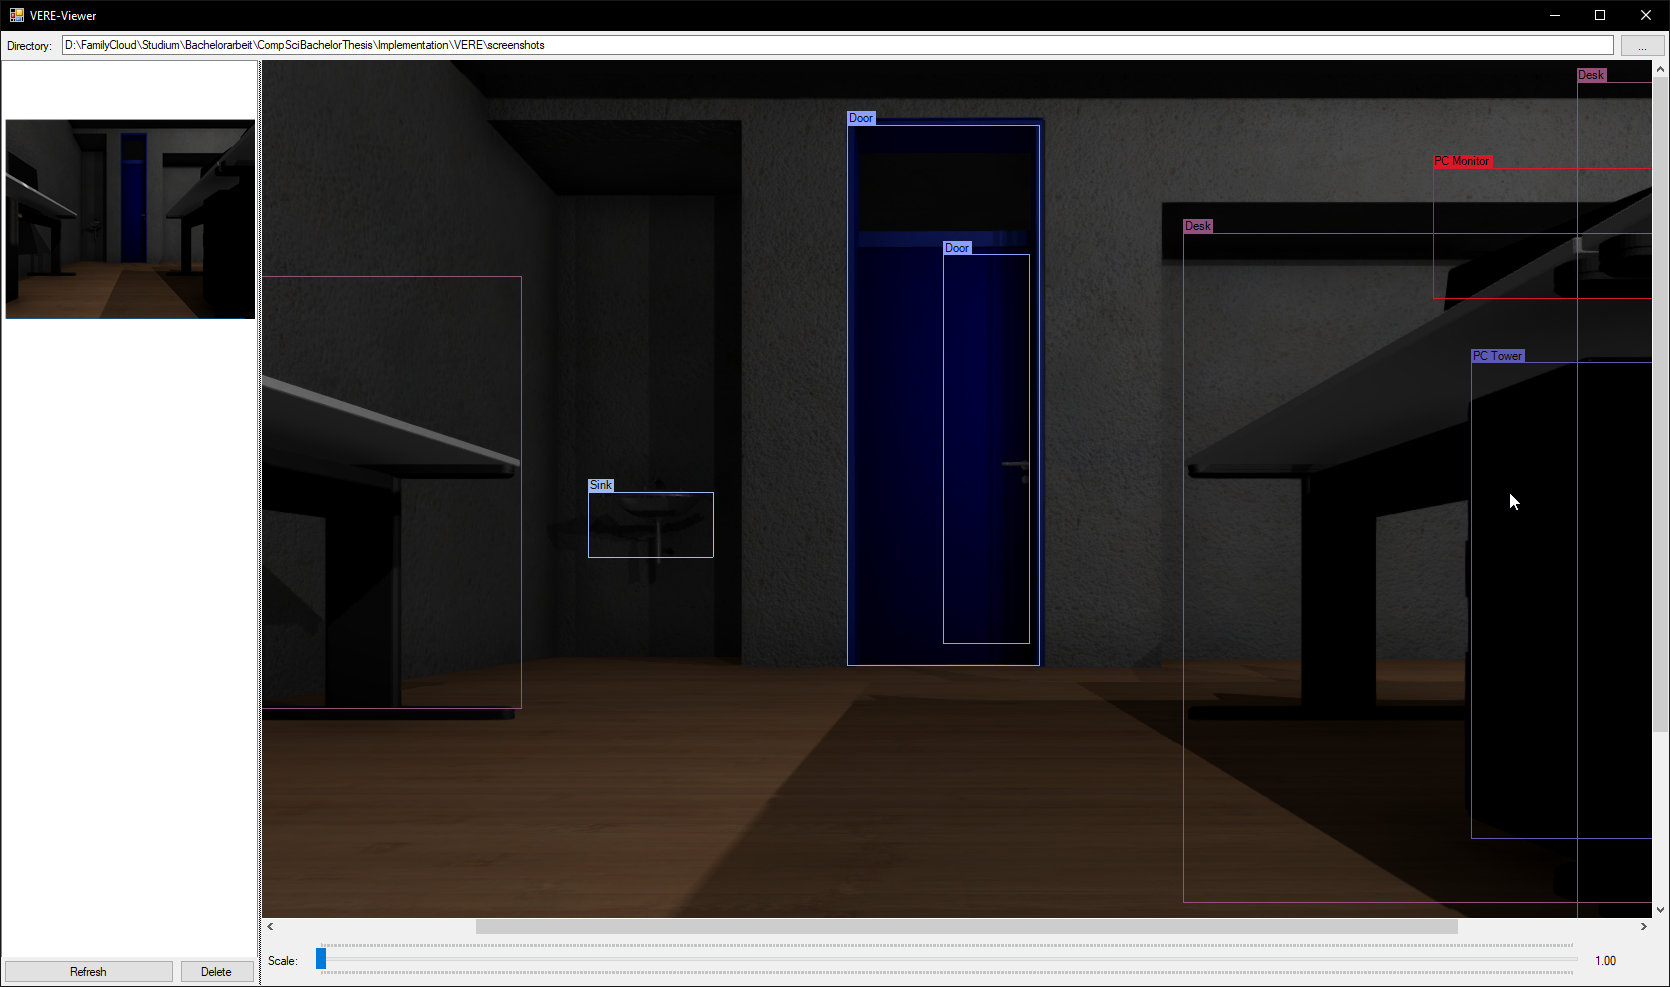
\includegraphics[height=350pt]{appendix/VERE-Viewer_2019-01-29.png}
    \captionof{figure}[Image in VERE-Viewer]{\ref{fig:output-image} and \ref{listing:output-meta} opened in VERE-Viewer}
    \label{fig:output-viewer}
\end{sidewaysfigure}